\documentclass[handout]{beamer}

% Lignes réponses
\usepackage{pgffor} % pour la commande \foreach permettant de réaliser une boucle
\newcommand{\pointilles}{{\\\rule{0pt}{1pt}\dotfill\rule{0pt}{1pt}}}
\newcommand{\rep}[1]{\foreach \n in {1,...,#1} {\pointilles}}

% Commandes pour cacher/révéler du texte facilement à l'aide d'un booléen
\usepackage{xstring}
\usepackage{ifthen}

\newboolean{reveal}
\setboolean{reveal}{false}

\newlength{\stextwidth} % une nouvelle longueur

\newcommand\x{6}

\newcommand{\guess}[1]{\ifthenelse{\boolean{reveal}}{{\color{red}#1}}{\settowidth{\stextwidth}{#1}\makebox[\stextwidth]{\dotfill}}}

\newcommand{\guessmath}[1]{\ifthenelse{\boolean{reveal}}{\textcolor{red}{#1}}{\settowidth{\stextwidth}{$#1$}\makebox[1.9\stextwidth]{\dotfill}}}

\newcommand{\guessmathbin}[1]{\ifthenelse{\boolean{reveal}}{\mathbin{\color{red}#1}}{\settowidth{\stextwidth}{$#1$}\makebox[2\stextwidth]{\dotfill}}}

% ========================================================================%

\usetheme{focus}

\usepackage{pgfpages}
\pgfpagesuselayout{4 on 1}[a4paper,landscape]

\usepackage[french]{babel}

\usepackage{xcolor}

\usepackage{pstricks,pst-plot,pst-text,pst-tree,pst-eps,pst-fill,pst-node,pst-math}
\usepackage{pstricks-add,pst-xkey}

\input ../tabvar

\usepackage{multicol}
\usepackage[np]{numprint}

\begin{document}

\title{}

\date{}

\begin{frame}
  \frametitle{Encadrer et arrondir un nombre réel}
  \textbf{Définition. --} \guess{Encadrer} un nombre réel $x$, c'est trouver deux nombres $a$ et $b$ tels que :
  \[\guessmathbin{a} \leq \guessmathbin{x} \leq \guessmathbin{b}\]
  $b-a$ est appelée l'\guess{amplitude} de l'encadrement.

  \begin{center}
    \psset{xunit=0.7cm,yunit=0.7cm,algebraic=true,dimen=middle,dotstyle=o,dotsize=10pt 0,linewidth=1.2pt,arrowsize=3pt 2,arrowinset=0.25}
    \begin{pspicture*}(1.,2.)(14.,5.)
      \psaxes[labelFontSize=\scriptstyle,xAxis=true,yAxis=true,Dx=1.,Dy=1.,ticksize=-2pt 0,subticks=2]{->}(0,0)(1.,2.)(14.,4.)
      \psline[linewidth=1.2pt](2.,3.)(13.,3.)
      \psdots[dotstyle=x](7.,3.)
      \psdots[dotstyle=x](5.,3.)
      \psdots[dotstyle=x](10.,3.)
      \psline{<->}(5,3.5)(10,3.5)
      \uput[u](7.5,3.5){Amplitude : $b-a$}
      \uput[d](5,3){$a$}
      \uput[d](7,3){$x$}
      \uput[d](10,3){$b$}
    \end{pspicture*}  
  \end{center}
\end{frame}

\begin{frame}
  \textit{Exemple. -- En utilisant la calculatrice (voir écran ci-dessous), on peut donner un encadrement d'amplitude $0,01$ de $\pi$ :
    \begin{center}
      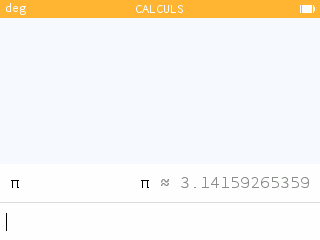
\includegraphics[width=6cm]{1_2_pi.png}
    \end{center}
  }
  \textit{On a :
    \[3,14\leq\pi\leq3,15.\]
  }
\end{frame}

\begin{frame}
\textit{On peut également arrondir $\pi$ à $10^{-2}$ près : \[\pi\approx3,14.\]
Plus précisément, l'arrondi de $\pi$ à $10^{-2}$ près est $3,14$.}

\medskip

\textit{Exemples. -- \begin{enumerate}
    \item Donner un encadrement de $\pi$ d'amplitude $10^{-6}$.
    \item Quel est l'arrondi de $\pi$ à $10^{-4}$ près ? à $10^{-8}$ près ?
\end{enumerate}}
\end{frame}

\begin{frame}
  \textit{\begin{enumerate}
      \setcounter{enumi}{2}
    \item En utilisant la calculatrice (voir écran ci-dessous), donner un encadrement de $\sqrt{2}$ d'amplitude $\np{0,001}$.
      \medskip
      \begin{center}
	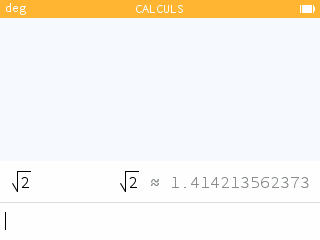
\includegraphics[width=6cm]{1_2_sqrt_2.png}
      \end{center}
      \medskip
    \item Donner l'arrondi de $\sqrt{2}$ à $\np{0,001}$ près.
\end{enumerate}}
\end{frame}

\end{document}

%%% Local Variables:
%%% mode: latex
%%% TeX-master: t
%%% End:
